% !TeX root = ./report.tex

本章将对 AGV 地图编辑器的功能进行详细的说明,将展示本软件完成的图例以及相应的代码说明。

\begin{figure}[H]
  \centering
  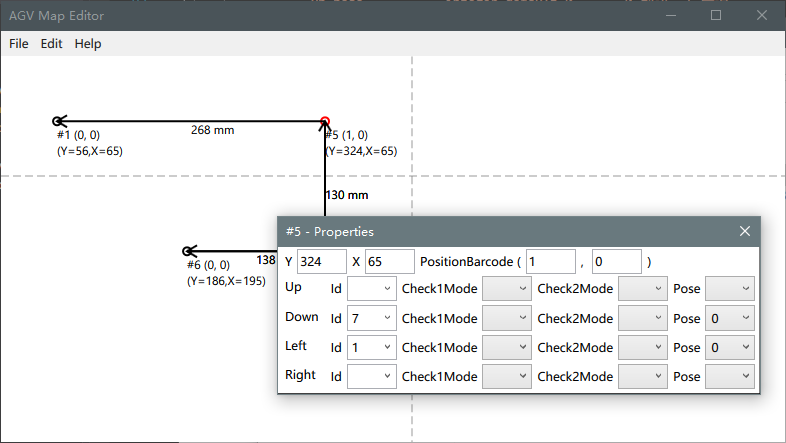
\includegraphics[width=0.8\textwidth]{assets/mainview.png}
  \caption{软件主界面}
  \label{fig:mainview}
\end{figure}

部分相关布局代码:

\begin{lstlisting}[language=XML]
<Window>
    <Grid>
        <InkCanvas EditingMode="None" />
        <Canvas>
            <Button Canvas.Top="10"
                    Canvas.Right="10"
                    Padding="10,5"
                    Content="Export SQL" />
            <Button Canvas.Right="10"
                    Canvas.Bottom="10"
                    Padding="10,5"
                    Content="Save" />
        </Canvas>
    </Grid>
</Window>
\end{lstlisting}

\section{启动}

首次启动本程序时,会自动从本程序所在同级目录下寻找 \texttt{MapData.db} 数据库文件并读取到程序内存。如果不存在该文件则会自动创建。如下图

\begin{figure}[H]
  \centering
  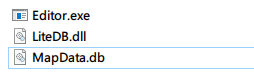
\includegraphics[width=0.4\textwidth]{assets/explorer.png}
  \caption{至少启动过一次后的程序文件夹}
  \label{fig:explorer}
\end{figure}

\section{创建坐标点}

移动鼠标,可以看到两条虚线分别对齐到鼠标的 XY 坐标上。此时在某一空白处双击即可创建新的坐标点。

\begin{figure}[H]
  \centering
  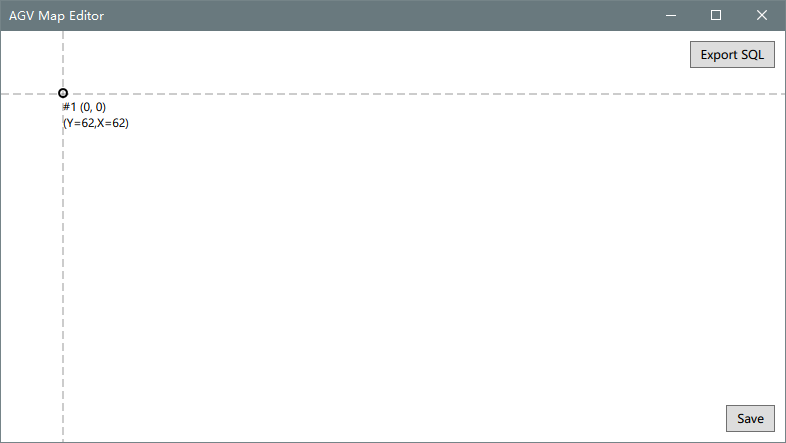
\includegraphics[width=0.8\textwidth]{assets/dbclick.png}
  \caption{在空白处双击后的界面}
  \label{fig:dbclick}
\end{figure}

坐标点的 ID 是自动分配的,不可以修改;XY 坐标赋值为鼠标位置,剩下的属性全都默认赋值为 0。同时可以注意到右下角出现了一个``保存''按钮,这个按钮我们下面再进行介绍。

相关代码:

\begin{lstlisting}[language=cs]
private void Window_MouseDoubleClick(object sender, MouseButtonEventArgs e) {
    if (/* click on the blank space */) {
        Map.Add(Cur = new Coord { X = CurX, Y = CurY });
        foreach (Coord c in Map) c.Update(ic, OffsetX, OffsetY);
        NeedSync = true;
    }
    // ... other stuff ...
}
\end{lstlisting}

\section{删除坐标点}

按下 \texttt{Delete} 即可删除当前被选中的坐标点,但用掉的编号不会再次变得可用。

相关代码:

\begin{lstlisting}[language=cs]
private void Ic_KeyUp(object sender, KeyEventArgs e) {
    if (e.Key == Key.Delete) {
        if (/* there be active point */) {
            Map.Remove(LastCur);
            foreach (Coord c in Map) {
                if (c.Up == LastCur) c.Up = null;
                if (c.Down == LastCur) c.Down = null;
                if (c.Left == LastCur) c.Left = null;
                if (c.Right == LastCur) c.Right = null;
            }
            LastCur.Remove(ic);
            LastCur = Cur = null;
            NeedSync = true;
        }
        sb.Visibility = NeedSync ? Visibility.Visible : Visibility.Hidden;
        RefreshMap();
    }
    // ... other stuff ...
}
\end{lstlisting}

\section{拖动坐标点}

直接在某个坐标点上按下鼠标左键,然后拖动即可,该点的 XY 坐标会跟着改变。默认情况下,拖动时会自动``吸附''到其他坐标点的四方向上,这时按住 Ctrl 可以取消吸附。代码中也体现了这一点。

相关代码:

\begin{lstlisting}[language=cs]
private void Ic_MouseMove(object sender, MouseEventArgs e) {
    Point pos = e.GetPosition(ic);
    double x = pos.X, y = pos.Y;
    if (IsPressingRight) {
        // ... other stuff ...
    } else {
        LastX = Double.NaN; LastY = Double.NaN;
        if (!IsPressingCtrl) {
            foreach (Coord c in Map) {
                if (c == Cur) continue;
                double cx = c.X + OffsetX, cy = c.Y + OffsetY;
                if (cx - 5 <= x && x <= cx + 5) x = cx;
                if (cy - 5 <= y && y <= cy + 5 && x != c.X) y = cy;
            }
        }
        CurX = x - OffsetX; CurY = y - OffsetY;
        HLine.MoveTo(0, y, ic.ActualWidth, y);
        VLine.MoveTo(x, 0, x, ic.ActualHeight);
        if (e.LeftButton == MouseButtonState.Pressed) {
            HLine.Hide();
            VLine.Hide();
            if (Cur != null && !PropertiesWindow.IsVisible) {
                Cur.X = CurX;
                Cur.Y = CurY;
                NeedSync = true;
            }
        } else {
            Cur = null;
            HLine.Show();
            VLine.Show();
        }
    }
    foreach (Coord c in Map) c.Update(ic, OffsetX, OffsetY);
    sb.Visibility = NeedSync ? Visibility.Visible : Visibility.Hidden;
}
\end{lstlisting}

\section{拖动画布}

按住鼠标右键然后拖动,整个画布会跟着一起移动,但是坐标点的坐标并不会改变。

相关代码:

\begin{lstlisting}[language=cs]
private void Ic_MouseMove(object sender, MouseEventArgs e) {
    Point pos = e.GetPosition(ic);
    double x = pos.X, y = pos.Y;
    if (IsPressingRight) {
        HLine.Hide();
        VLine.Hide();
        if (Double.IsNaN(LastX)) {
            LastX = x; LastY = y;
        } else {
            OffsetX += x - LastX;
            OffsetY += y - LastY;
            LastX = x; LastY = y;
        }
    } else {
        // ... other stuff ...
    }
    foreach (Coord c in Map) c.Update(ic, OffsetX, OffsetY);
    sb.Visibility = NeedSync ? Visibility.Visible : Visibility.Hidden;
}
\end{lstlisting}

\section{修改坐标点属性}

在一个坐标点上双击,即可打开``属性''窗口。

\begin{figure}[H]
  \centering
  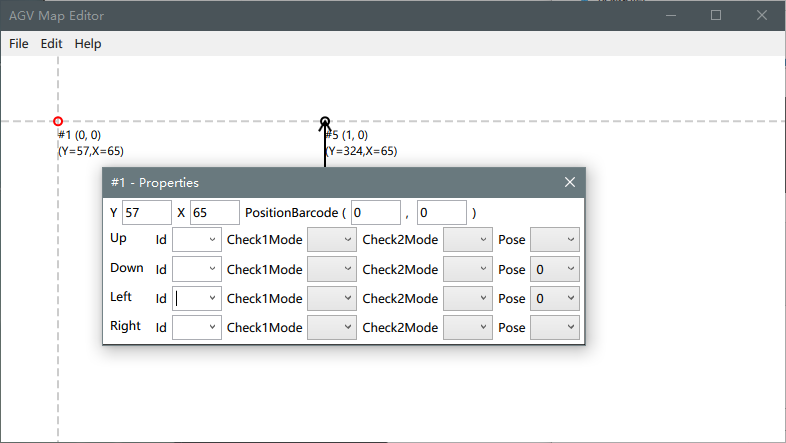
\includegraphics[width=0.8\textwidth]{assets/prop.png}
  \caption{``属性''窗口}
  \label{fig:prop}
\end{figure}

接下来我们尝试给 \#1 坐标点加一个指向 \#2 的路径,在 Right Id 下拉框中选中 2:

\begin{figure}[H]
  \centering
  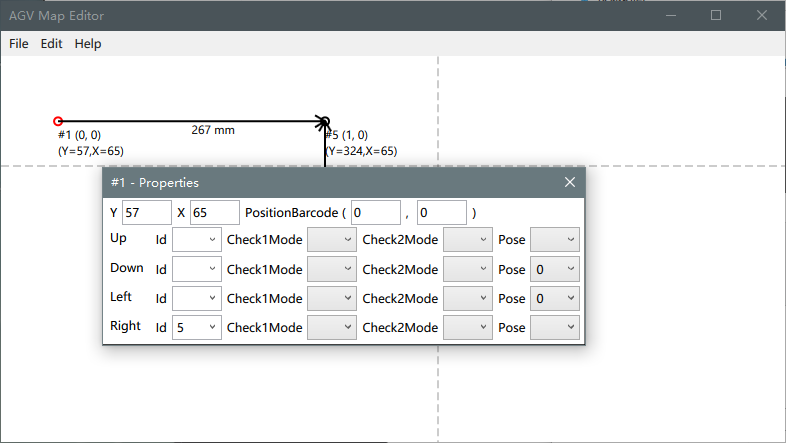
\includegraphics[width=0.8\textwidth]{assets/prop2.png}
  \caption{``属性''窗口}
  \label{fig:prop2}
\end{figure}

可以看到界面立刻产生了变化。

这个属性编辑窗口的内容改变是直接写回内存的,所以没有相关``保存''按钮。编辑完直接关掉即可。

相关代码(部分):

\begin{lstlisting}[language=XML]
<Window>
    <StackPanel Margin="2">
        <WrapPanel Grid.ColumnSpan="2">
            <Label Content="Y" />
            <TextBox Name="X" TextChanged="X_TextChanged" />
            <Label Content="X" />
            <TextBox Name="Y" TextChanged="Y_TextChanged" />
            <Label Content="PositionBarcode (" />
            <TextBox Name="I" TextChanged="I_TextChanged" />
            <Label Content=", " />
            <TextBox Name="J" TextChanged="J_TextChanged" />
            <Label Content=")" />
        </WrapPanel>
        <Grid>
            <Grid.RowDefinitions>
                <RowDefinition Height="*" />
                <RowDefinition Height="*" />
                <RowDefinition Height="*" />
                <RowDefinition Height="*" />
            </Grid.RowDefinitions>
            <Grid.ColumnDefinitions>
                <ColumnDefinition Width="Auto" />
                <ColumnDefinition Width="Auto" />
            </Grid.ColumnDefinitions>
            <Label Grid.Row="0" Content="Up" />
            <StackPanel Orientation="Horizontal" Grid.Row="0" Grid.Column="2" Margin="2">
                <Label Content="Id" />
                <ComboBox Name="UpId" SelectionChanged="UpId_SelectionChanged" >
                    <ComboBoxItem Content="" />
                </ComboBox>
                <Label Content="Check1Mode" />
                <ComboBox Name="UpCheck1Mode" SelectionChanged="UpCheck1Mode_SelectionChanged">
                    <ComboBoxItem Content="" />
                    <ComboBoxItem Content="1" />
                    <ComboBoxItem Content="2" />
                    <ComboBoxItem Content="3" />
                    <ComboBoxItem Content="4" />
                    <ComboBoxItem Content="5" />
                    <ComboBoxItem Content="6" />
                    <ComboBoxItem Content="7" />
                </ComboBox>
                <Label Content="Check2Mode" />
                <ComboBox Name="UpCheck2Mode" SelectionChanged="UpCheck2Mode_SelectionChanged">
                  <!-- same as check1mode -->
                </ComboBox>
                <Label Content="Pose" />
                <ComboBox Name="UpPose" SelectionChanged="UpPose_SelectionChanged">
                    <ComboBoxItem Content="0" />
                    <ComboBoxItem Content="1" />
                </ComboBox>
            </StackPanel>
            <!-- other rows -->
        </Grid>
    </StackPanel>
</Window>
\end{lstlisting}

\begin{lstlisting}[language=cs]
public Coord Coord {
    get => Coord_;
    set {
        Coord_ = null;
        X.Text = ((int)value.X).ToString();
        Y.Text = ((int)value.Y).ToString();
        I.Text = value.I.ToString();
        J.Text = value.J.ToString();
        if (value.Up != null) {
            for (int i = 1; i < UpId.Items.Count; i++) {
                if (Ids[i - 1] == value.Up.Id) {
                    UpId.SelectedIndex = i;
                    break;
                }
            }
            UpCheck1Mode.SelectedIndex = (value.M_Up & 0b01110000) >> 4;
            UpCheck2Mode.SelectedIndex = (value.M_Up & 0b00001110) >> 1;
            UpPose.SelectedIndex = value.M_Up & 0b00000001;
        } else {
            UpId.SelectedIndex = 0;
        }
        // down, left, right
        Coord_ = value;
    }
}

private List<Coord> Map;
private int[] Ids;

private void X_TextChanged(object sender, TextChangedEventArgs e) {
    if (Coord_ == null) return;
    if (Int32.TryParse(X.Text, out int _x)) {
        Coord_.X = _x;
    } else {
        X.Text = ((int)Coord_.X).ToString();
    }
}

private void Y_TextChanged(object sender, TextChangedEventArgs e) {
    if (Coord_ == null) return;
    if (Int32.TryParse(Y.Text, out int _y)) {
        Coord_.Y = _y;
    } else {
        Y.Text = ((int)Coord_.Y).ToString();
    }
}

// other fields...
\end{lstlisting}

篇幅有限,代码均做了大量精简。

\section{保存到数据库}

点击右下角的``保存''按钮,即将数据写入数据库。

\begin{figure}[H]
  \centering
  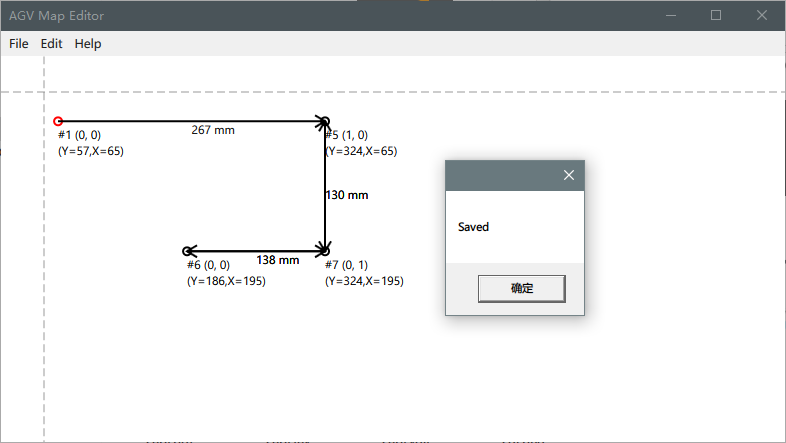
\includegraphics[width=0.8\textwidth]{assets/save.png}
  \caption{保存成功对话框}
  \label{fig:save}
\end{figure}

相关代码:

\begin{lstlisting}[language=cs]
private void Sb_Click(object sender, RoutedEventArgs e) {
    sb.Content = "Saving...";
    foreach (Coord c in Map) c.UpdateNeighbours();
    using (LiteDatabase db = new LiteDatabase("./MapData.db")) {
        db.DropCollection("map");
        LiteCollection<Coord> map = db.GetCollection<Coord>("map");
        map.EnsureIndex(c => c.Id);
        map.InsertBulk(Map);
    }
    MessageBox.Show("Saved");
    NeedSync = false;
    sb.Visibility = Visibility.Hidden;
    sb.Content = "Save";
}
\end{lstlisting}

\section{导出 SQL}

点击右上角的``导出 SQL''按钮,即将数据输出成 SQL 语句的形式。

\begin{figure}[H]
  \centering
  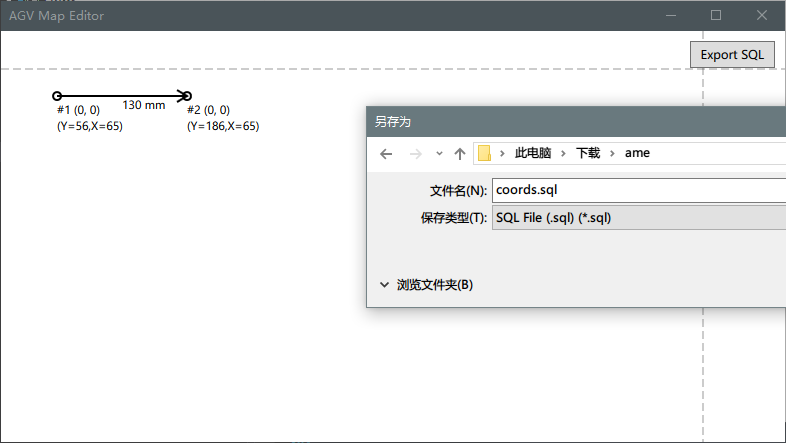
\includegraphics[width=0.8\textwidth]{assets/export.png}
  \caption{导出到 SQL 文件对话框}
  \label{fig:export}
\end{figure}

按确定后会在目标位置生成 SQL 文件,里面包含了创建和插入表的 SQL 语句。

\begin{figure}[H]
  \centering
  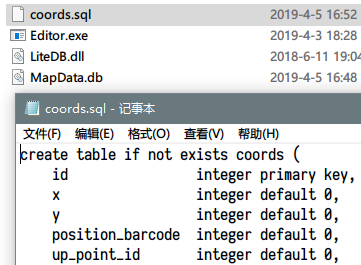
\includegraphics[width=0.5\textwidth]{assets/sql.png}
  \caption{SQL 文件内容}
  \label{fig:sql}
\end{figure}

部分相关代码:

\begin{lstlisting}[language=cs]
public string ToSql => $@"insert into coords values (
    {Id}, {(int)X}, {(int)Y}, {(I << 16) | J},
    {UpId}, {(M_Up & 0b01110000) >> 4}, {(M_Up & 0b00001110) >> 1}, {(M_Up & 0b00000001)},
    {DownId}, {(M_Down & 0b01110000) >> 4}, {(M_Down & 0b00001110) >> 1}, {(M_Down & 0b00000001)},
    {LeftId}, {(M_Left & 0b01110000) >> 4}, {(M_Left & 0b00001110) >> 1}, {(M_Left & 0b00000001)},
    {RightId}, {(M_Right & 0b01110000) >> 4}, {(M_Right & 0b00001110) >> 1}, {(M_Right & 0b00000001)}
)";

private void Es_Click(object sender, RoutedEventArgs e) {
    StringBuilder builder = new StringBuilder(Coord.ToTableSql);
    foreach (Coord c in Map) {
        builder.Append(c.ToSql);
        builder.Append(';');
    }
    string result = builder.ToString();
    SaveFileDialog dialog = new SaveFileDialog {
        FileName = "coords",
        DefaultExt = ".sql",
        Filter = "SQL File (.sql)|*.sql|Text documents (.txt)|*.txt"
    };
    if (dialog.ShowDialog() == true) {
        File.WriteAllText(dialog.FileName, result);
    }
}
\end{lstlisting}
